\documentclass{article}
\usepackage[T1]{fontenc}
\usepackage{tgbonum}
\usepackage[english]{babel}
\usepackage[letterpaper,top=2.5cm,bottom=2.5cm,left=2.5cm,right=2.5cm,marginparwidth=1.75cm]{geometry}

% Useful packages
\usepackage{amsmath}
\usepackage{graphicx}
\usepackage[colorlinks=true, allcolors=blue]{hyperref}

\title{IMAGine Instruction Set}
\author{MD Arafat Kabir}

\begin{document}
\maketitle


\section{IMAGine Architecture}
This is a very brief introduction to IMAGine's high-level architecture.
IMAGine is a GEMV accelerator consisting of two submodules: the GEMV array
and the column-shift-registers.
In Fig.~\ref{fig:archSysTile}~(a), shows these modules.
The interface to IMAGine are two FIFOs.
You push your instructions through the FIFO-in, and
IMAGine pushes out the output through the FIFO-out.
The output needs to be stored in the column-shift-registers before
they can be pushed to the FIFO-out.


\begin{figure}[h]
\centering
%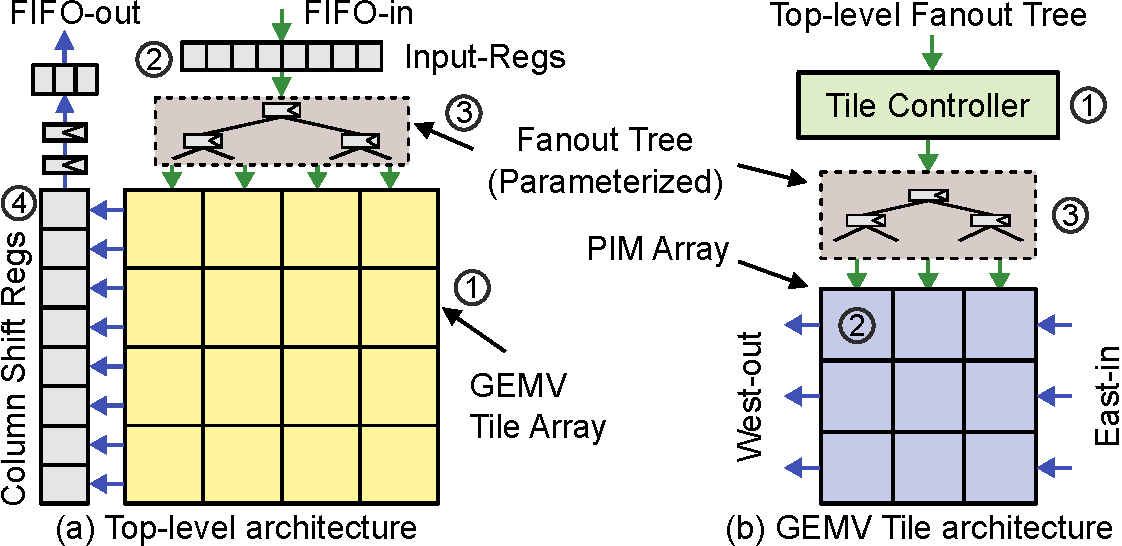
\includegraphics[width=\linewidth]{fig/sys-tile-arch.png}
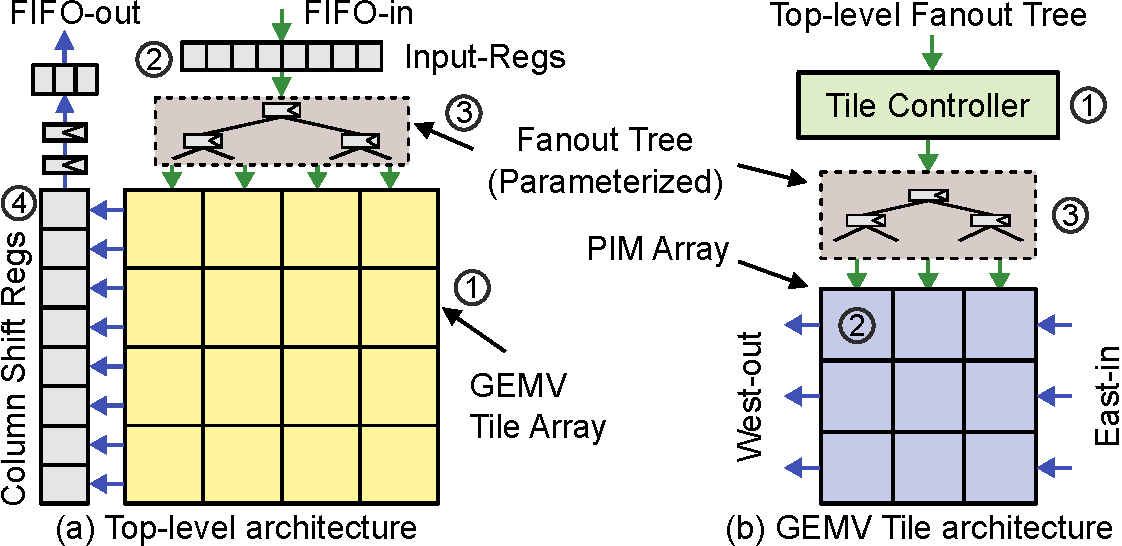
\includegraphics[width=0.7\linewidth]{fig/sys-tile-arch.pdf}
\caption{
System architecture of IMAGine
(a) GEMV engine (\texttt{mv\_}) \& column-shift-register (\texttt{vv\_}) submodules,
(b) Architecture of a GEMV tile.
}
\label{fig:archSysTile}
\end{figure}


\begin{figure}[h]
\centering
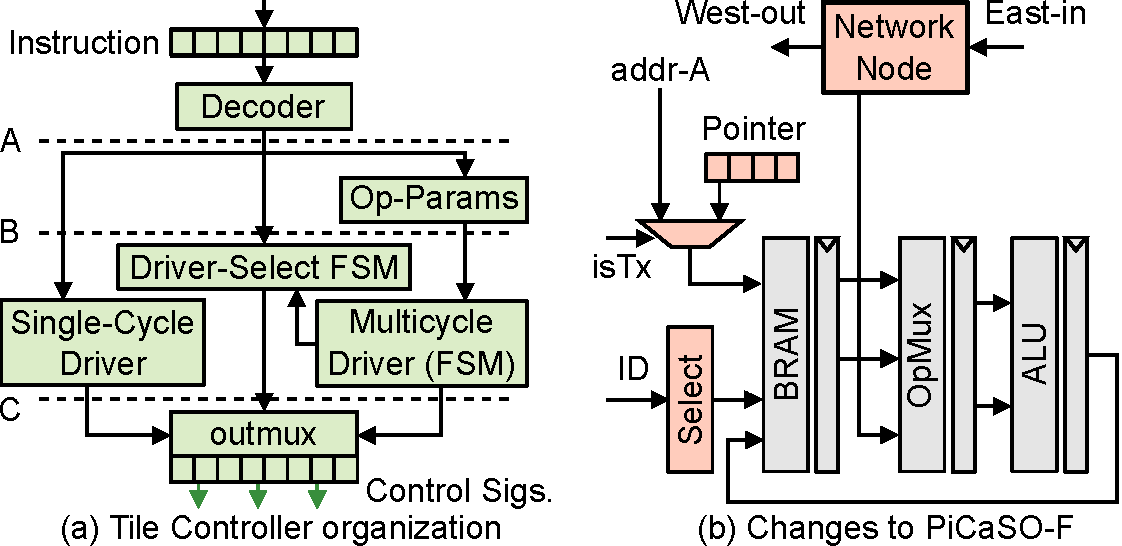
\includegraphics[width=0.7\linewidth]{fig/control-pim-arch.pdf}
\caption{
Architectures of 
(a) GEMV controller and 
(b) PIM block (PiCaSO-IM).
}
\label{fig:archControlPim}
\end{figure}


\section{Built-in Instructions}
These are instructions built into IMAGine. 
Each instruction mnemonic generates exactly one instruction word. 
However, some instruction may be executed by the hardware in multiple cycles.
Instructions prefixed with \texttt{mv\_} are dispatched to the GEMV array submodule and the
instructions prefixed with \texttt{vv\_} are dispatched to the column-shift-register submodule.
Submodules can concurrently execute their instructions unless a synchronization barrier is used.

The register arguments (e.g. rs1, rs2, rd, reg, etc.) are integers greater than 0.
The largest value of the integer arguments depends on the assembler parameters and the instruction.
The optional keyword argument \texttt{comment} after * can be used to emit user comments in the
outputs generated by the export directives.
Other keyword arguments (e.g. skipChekcs) after * can be safely ignored for programming purposes.


\subsubsection*{mv\_write (self, addr, data, *, comment=None)}
This is a single-cycle instruction for the GEMV array.
Writes the \texttt{data} at the \texttt{addr} of the BRAM (PiCaSO) block(s)
currently selected.
Use one of the select instructions to select the BRAM before write:
\texttt{mv\_selectBlk},
\texttt{mv\_selectRow},
\texttt{mv\_selectCol}, and
\texttt{mv\_selectAll}.


\subsubsection*{mv\_nop (self, *, comment=None)}
This is a single-cycle instruction that generates a NOP for the GEMV array.
This effectively consumes one cycle without changing internal state.


\subsubsection*{mv\_mov (self, rd, rs, *, comment=None)}
This is a multicycle instruction for the GEMV array.
It moves (copies) the contents of the \texttt{rs} register into the \texttt{rd}
register.


\subsubsection*{mv\_add (self, rd, rs1, rs2, *, comment=None)}
This is a multicycle instruction for the GEMV array.
It adds the contents of the registers \texttt{rs1} and \texttt{rs2}
and stores the resutl in the register \texttt{rd}. 
This is effectively $rd = rs1 + rs2$.


\subsubsection*{mv\_sub (self, rd, rs1, rs2, *, comment=None)}
This is a multicycle instruction for the GEMV array.
It the contents of \texttt{rs2} from \texttt{rs1}
and stores the resutl in the register \texttt{rd}. 
This is effectively $rd = rs1 - rs2$.


\subsubsection*{mv\_movOffset (self, offset, rd, rs, *, comment=None, skipChecks=False)}
This is a multicycle instruction for the GEMV array.
It moves (copies) the contents of the \texttt{rs} register, starting at bit
position \texttt{offset}, into the \texttt{rd} register.
This instruction does not respect the register boundary.
This means, the upper bits of \texttt{rd} will contain \texttt{offset} number
of lower bits of the \texttt{rs+1}-th register.
This instruction is used after multiplication to perform right-shift of the multiplication
result stored in two consecutive registers.


\subsubsection*{mv\_selectBlk (self, rowID, colID, *, comment=None)}
This is a single-cycle instruction to select a single PiCaSO block for
selective operations like \texttt{mv\_write}.
To select a specific block both \texttt{rowID} and \texttt{colID} are needed.


\subsubsection*{mv\_selectRow (self, rowID, *, comment=None)}
This is a single-cycle instruction to select all PiCaSO blocks in an entire row
of the GEMV array for selective operations like \texttt{mv\_write}.
Only \texttt{rowID} is needed for the row selection.


\subsubsection*{mv\_selectCol (self, colID, *, comment=None)}
This is a single-cycle instruction to select all PiCaSO blocks in an entire column
of the GEMV array for selective operations like \texttt{mv\_write}.
Only \texttt{rowID} is needed for the row selection.


\subsubsection*{mv\_selectAll (self, *, comment=None)}
This is a single-cycle instruction to select all PiCaSO blocks in the GEMV
array for selective operation like \texttt{mv\_write}.


\subsubsection*{mv\_updatepp (self, ppreg, multiplicand, multiplier, bitNo, *, comment=None)}
This is a multicycle instruction to update the partial-product based on the
\texttt{bitNo}-th bit of the multiplier.
The result is equivalent of, \\
\texttt{
\hspace*{1cm} ppreg[bitNo +: N] += multiplicand * multiplier[bitNo]; // N = register width \\
\hspace*{1cm} ppreg[bitNo + N] = ppreg[bitNo + N - 1]; // Sign extension
}


\subsubsection*{mv\_blockFold (self, fold, rd, rs, *, comment=None)}
This is a multicycle instruction to add a fold of \texttt{rs} with itself
and store the result in the destination register \texttt{rd}.
Here, \texttt{rd} and \texttt{rs} can be the same register.
The result is equivalent of, \\
\hspace*{1cm} \texttt{rd = rs + folded(rs, fold)}.


\subsubsection*{mv\_accumRow (self, level, reg, *, comment=None)}
This is a multicycle instruction to add the block-level accumulation result
of different blocks in a row based on the accumulation tree \texttt{level}.
The result is equivalent of, \\
\hspace*{1cm} \texttt{receiver-pe0-reg += transmitter-pe0-reg}


\subsubsection*{vv\_nop (self, *, comment=None)}
This is a single-cycle instruction that generates a NOP for the
column-shift-register submodule.
This effectively consumes one cycle without changing internal state.


\subsubsection*{vv\_shiftOff (self, *, comment=None)}
This is a single-cycle instruction that turns off all types of shifting in the
column-shift-register submodule.


\subsubsection*{vv\_serialEn (self, *, comment=None)}
This is a single-cycle instruction that enables serial shifting from GEMV array into the
column-shift-register submodule.
This automatically disables parallel shifting.


\subsubsection*{vv\_parallelEn (self, *, comment=None)}
This is a multicycle instruction that enables parallel shifting from GEMV array into the
column-shift-register submodule.
This automatically disables serial shifting.




\section{Assembler Macros}
These are high-level macro-instructions provided by the assembler, built on top
of the built-in instructions.
Each instruction mnemonic exapands into several (sometimes hundreds) built-in
instruction words.
The programmers are encouraged to use the macros as much as possible to avoid
the intricacies of the built-in instructions.


\subsubsection*{mv\_MULT (self, rd, multiplicand, multiplier, *, comment=None, skipChecks=False)}
This instruction performs signed multiplication between the registers \texttt{multiplicand} and
\texttt{multiplier} using the \texttt{mv\_updatepp} built-in instruction.
The result is stored spanning two registers \texttt{\{rd, rd+1\}}.


\subsubsection*{mv\_MULTFXP (self, rd, multiplicand, multiplier, *, comment=None)}
This instruction performs signed fixed-point multiplication between the
registers \texttt{multiplicand} and \texttt{multiplier} using the
\texttt{mv\_updatepp} and \texttt{mv\_movOffset} built-in instructions.
This instruction depends on the assembler parameter \texttt{fracWidth} and
reserved registers.


\subsubsection*{mv\_SYNC (self, *, comment=None)}
This is a synchronization barrier for the GEMV array.
Next instruction will not be fetched and executed until the last \texttt{mv\_}
instruction finishes.
This instruction can be used to stall the execution of an instruction on the
column-shift-register submodule, which needs the result of the last instruction
dispatched to the GEMV array submodule.


\subsubsection*{vv\_SYNC (self, *, comment=None)}
This is a synchronization barrier for the column-shift-register submodule.
Next instruction will not be fetched and executed until the last \texttt{vv\_}
instruction finishes.
This instruction can be used to stall the execution of an instruction on the
GEMV array submodule, which needs the last instruction dispatched to the
column-shift-register to finish first.


\subsubsection*{mv\_BLOCKACCUM (self, rd, rs, *, comment=None)}
This instruction performs the block-level accumulation of the \texttt{rs}
register and saves the result in the \texttt{rd} register using the
\texttt{mv\_blockFold} built-in instruction.


\subsubsection*{mv\_RNGACCUM (self, colCnt, rd, rs, *, comment=None)}
This instruction accumulates the \texttt{rs} register of PE columns (0 :
colCnt-1) into \texttt{rd} register using a combination of \texttt{mv\_blockFold}
and \texttt{mv\_accumRow}.


\subsubsection*{mv\_ALLACCUM (self, rd, rs, *, comment=None)}
This instruction accumulates the \texttt{rs} register of all PE columns in a
row into \texttt{rd} register using a combination of \texttt{mv\_blockFold} and
\texttt{mv\_accumRow}.


\subsubsection*{mv\_CLRREG (self, reg, *, comment=None)}
This instruction clears the register \texttt{reg} by writing zeros to the
corresponding rows of the BRAM block.


\subsubsection*{mv\_LOADMAT (self, reg, matrix, *, comment=None)}
This instruction generates instruction to load a floating-point (or integer)
matrix into the register \texttt{reg} of the GEMV array.

It performs the necessary bit-manipulations to convert the floating-point (or integer)
values to transposed bit-patterns for the corresponding fixed-point representation.
It is compatible with numpy, i.e, the \texttt{matrix} can be a numpy ndarray instance.
This macro is data aware: it generates the instructions to clear the register
first and then write only the non-zero rows to the target BRAMs.
Thus, if a matrix with all zeros is loaded, it only clears the register.


\subsubsection*{mv\_LOADVEC\_ROW (self, reg, vector, *, comment=None)}
This instruction generates instruction to load a floating-point (or integer)
row-vector into the register \texttt{reg} of the GEMV array.
The same vector is loaded into all rows of the GEMV array.

It performs the necessary bit-manipulations to convert the floating-point (or integer)
values to transposed bit-patterns for the corresponding fixed-point representation.
It is compatible with numpy, i.e, the \texttt{vector} can be a numpy ndarray instance.
This macro is data aware: it generates the instructions to clear the register
first and then write only the non-zero rows to the target BRAMs.
It takes advantage of the broadcast network connected to the GEMV array to 
write to all rows at the same time.
Thus, it is a better choice than \texttt{mv\_LOADMAT} if a matrix needs to be
loaded which has identical rows.



\subsubsection*{mv\_LOADVEC\_COL (self, reg, vector, *, comment=None)}
This instruction generates instruction to load a floating-point (or integer)
column-vector into the register \texttt{reg} of the GEMV array.
The same vector is loaded into all columns of the GEMV array.

It performs the necessary bit-manipulations to convert the floating-point (or integer)
values to transposed bit-patterns for the corresponding fixed-point representation.
It is compatible with numpy, i.e, the \texttt{vector} can be a numpy ndarray instance.
This macro is data aware: it generates the instructions to clear the register
first and then write only the non-zero rows to the target BRAMs.
It takes advantage of the broadcast network connected to the GEMV array to 
write to all columns at the same time.
Thus, it is a better choice than \texttt{mv\_LOADMAT} if a matrix needs to be
loaded which has identical columns.




\section{Assembler Directives}
These are assembler directives to control various aspects of the assembly and
instruction generation process.



\subsubsection*{setupParams (self, regCnt, regWidth, maxLevel, maxFold, idWidth, fracWidth, mvBlockDim, resvRegCnt)}
This directive sets up the assembler parameters.
The assembly programmers should avoid using this function directly and use the \texttt{loadParams()}
directive instead to load the appropriate parameters.
Default values of the parameters are, \\
\hspace*{1cm} regCnt = 16, regWidth = 16, maxLevel = 3, maxFold = 4, \\
\hspace*{1cm} idWidth = 8, fracWidth = 0, mvBlockDim = None, resvRegCnt = 0


\subsubsection*{loadParams (self, filepath, cpright=True, showparams=True)}
This directive loads the assembler parameters from and external YAML file.


\subsubsection*{reset (self)}
This directive resets the internal state of the assembler and clears the
instruction cache, without affecting the assembler parameters.
This directive should be called before starting a new program and after exporting 
the previous program in a multi-program assembler script.


\subsubsection*{assemble (self, verbose=False)}
This directive assembles the instructions in the instruction cache and convert
them into their machine-code representation.
It does not generate any output, only updates the internal state of the
assembler.
It is usually not necessary to be called directly by the programmer.
Any of the export directives will implicitly call it if there is even a single
unassembled instruction in the cache.


\subsubsection*{export\_verilogBin (self, filename=None, comment=True, source=True, separator='\_')}
This directive exports the assembled instructions as binary string with the \texttt{separator}
between the instruction word fields.
The exported output can be used in Verilog/SystemVerilog simulation tools using
the \$readmemb() system task.


\subsubsection*{export\_CprogHex (self, progname, filename=None, comment=True, source=True)}
This directive exports the assembled instructions as unsigned hex number C-array.
The exported output can be compiled into object code using a C compiler to be
used in the application program, along with necessary header files.


\subsubsection*{export\_CprogHeader (self, filename=None)}
This directive exports a C-header file containing the definition of the struct
that can hold all the necessary information and the compiled instructions.


\subsubsection*{as\_addComment (self, comment)}
This directive looks like an instruction and can be used to emit comments in
the outputs generated by the export directives.


\end{document}


